\section{Additional Experiment Details}
\label{app:exp_details}

\subsection{Hierarchical Bayes Evaluation}
We sample $M$ linear models according to the hierarchical model in Section~\ref{sec:hierarchical_bayes}, with design matrices constructed by uniformly sampling points, $x \sim U[-1,1]$, and storing the vector $\bx_j = x^j$, for $i=0,\ldots,d$ in each row of $\DXi{i}$.

To produce the plots in Figure~\ref{fig:hierarchical_lreg_simulation} we computed the average loss over 100 random draws of the training data and labels from the same set of fixed $\btheta_{1:M+1}$ values. The $\btheta$ values were sampled once from the hierarchical model with $\tau = [0, 1, 2, 0, 0, 3, 1]$, and $\sigma^2_\theta = 0.1$

Code to reproduce these plots is provided in the supplementary materials with our submission.

\subsection{Sinusoid Regression with MAML}

% \subsection{Sinusoid regression with MAML}

Following the connections between MAML and hierarchical Bayes explored by \citet{grant2018recasting}, we also explored regression on sinusoids using MAML. Our aim was to investigate how predictive our linear theory is for this highly non-linear problem setting. As in \citet{finn2017model}, we sample sinusoid functions by placing a prior over the amplitude and phase. In other works \citep{finn2017model, grant2018recasting} the same prior is used for the training and testing stages. However, to better measure generalization to novel tasks we use different prior distributions when training versus evaluating the model.

\iflatexml
\begin{figure}
    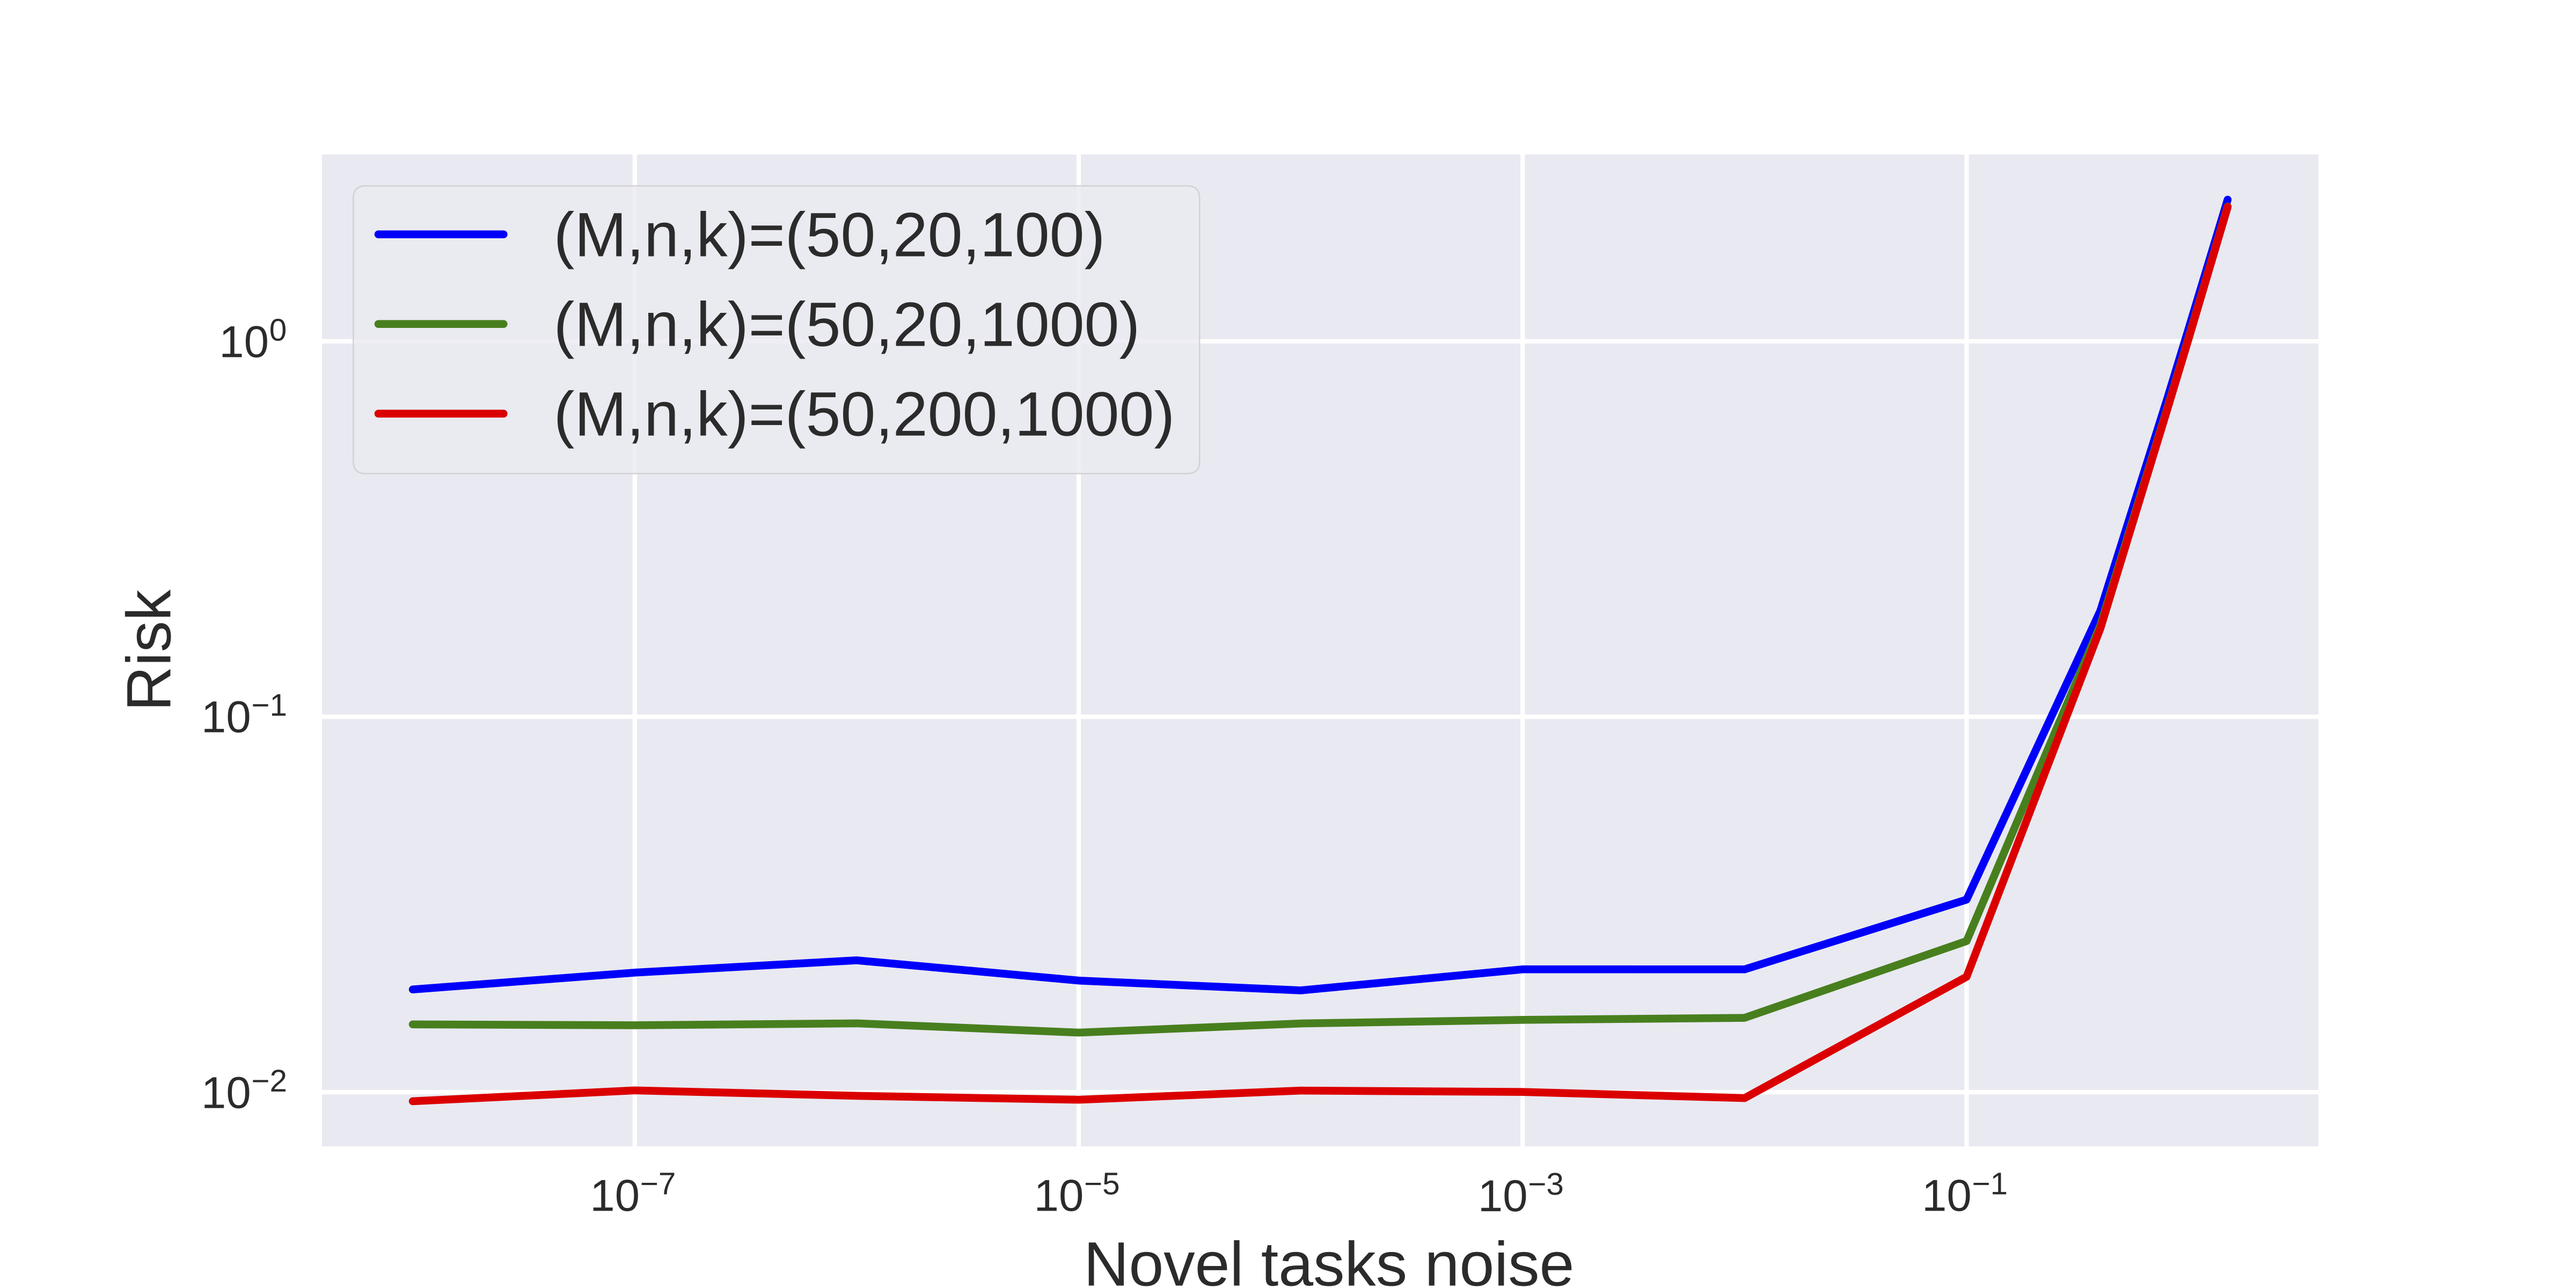
\includegraphics[width=4\linewidth]{main/images/maml_sinusoid.png}
  \caption{Average risk for regressing sinusoid functions with MAML.}
  \label{fig:maml_sinusoid}
\end{figure}
\else
\begin{wrapfigure}{r}{0.48\textwidth}
  \begin{center}
    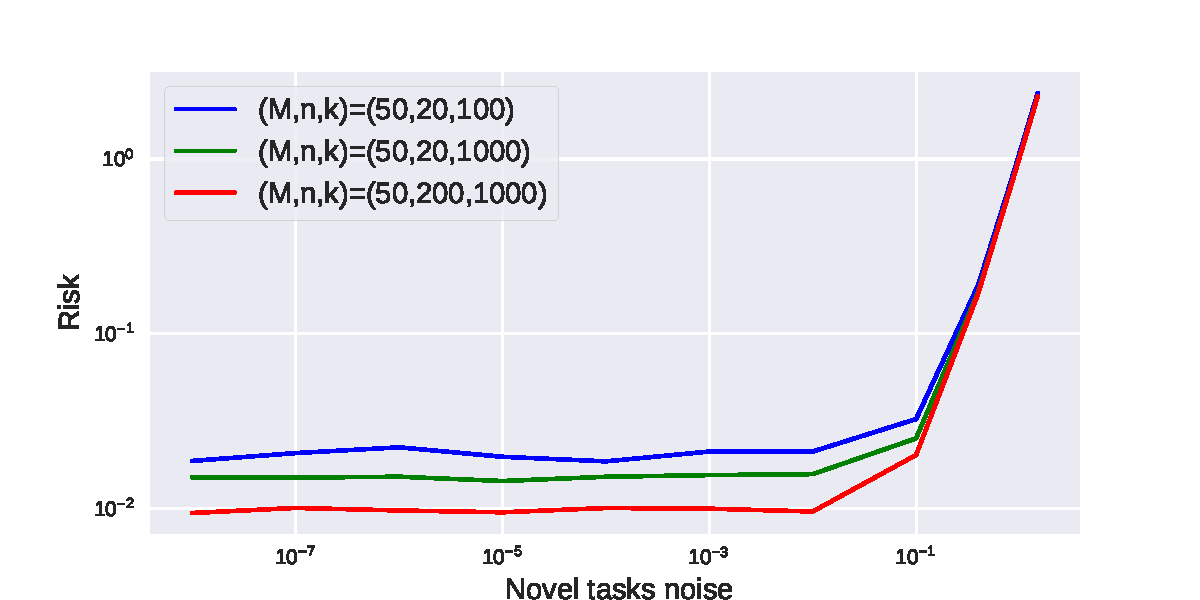
\includegraphics[width=0.48\textwidth]{main/images/maml_sinusoid.pdf}
  \end{center}
  \caption{Average risk for regressing sinusoid functions with MAML.}
  \label{fig:maml_sinusoid}
\end{wrapfigure}
\fi

We display the risk averaged over 30 trials in Figure~\ref{fig:maml_sinusoid}. We varied the novel task difficulty by increasing the observation noise in the novel task.
We plot separate curves for different dataset size configurations, and observe that the empirical results align fairly well with the results derived by sampling the hierarchical model (Figure \ref{fig:hierarchical_lreg_simulation}A). Adding more meta-training data (increasing $n$) is beneficial (green vs. yellow)
and adding more test data-points (higher $k$) is also beneficial (red vs. green).  Here however, these relationships did not interact with the task difficulty, as the wins for increased meta-training and meta-testing data were consistent, until task noise prevents any setting of the model from performing the task.


\begin{table}[H]
    \centering
    \begin{tabular}{l|c}
    Hyper parameters & Description \\
    \hline
    $\sigma$ & noise at test time.\\
    M & number of tasks at the training tasks\\
    $M_q$     & number of tasks at the testing tasks \\
    eps\_per\_batch & episode per batch          \\
    train\_ampl\_range &    range of amplitude at training          \\
    train\_phase\_range &  range of phase at training \\
    val\_ampl\_range &  range of amplitude  at testing \\
    val\_phase\_range & range of phase at testing\\
    inner\_steps &  number of steps of Maml  \\
    inner\_lr &  learning rate used to optimize parameter of the model \\
    meta\_lr & used to optimize parameter of the meta-learner \\
    n & number of datapoints at training tasks(support set) \\
    k & number of datapoints at testing  tasks (support set)\\

    $n_q$ &  number of datapoints at training  tasks (query set)  .\\
    $k_q$ & number of datapoints at testing  tasks (query set).\\
    
    \end{tabular}
\end{table}

%\subsubsection{Sinusoid Regression on sinusoids with MAML: Experiment design}

For all of these experiments we used a fully connected network with 6 layers and 40 hidden units per layer. The network is trained using the MAML algorithm \citep{finn2017model} with 5 inner steps using SGD with an inner learning rate of $10^{-3}$. We used Adam for the outer loop learning with a learning rate of $10^{-3}$.


Expected error was computed after 500 epochs of optimization and was averaged over 30 runs. We produced our results through a comprehensive grid search over 72 combinations of the settings below and it required around 30 minutes to produce the output of each setting, using a system with 1 gpu and 3 cpus. This experiment therefore lasted 20 hours in total.
\\
\iflatexml
$M=50$, $n \in \{20, 200\}$, $k \in \{100,1000\}$,
$\sigma \in [ 10^{-8}, 1.5]$,
$M_q = 100$, 
eps\_per\_batch = $25$,
train\_ampl\_range = $[1,4]$,
train\_phase\_range = $[0, \pi / 2 ]$,
val\_ampl\_range = $[3,5]$,
val\_phase\_range = $[0, \pi / 2 ]$,
inner\_steps = $5$,
inner\_lr = $10^{-3}$,
meta\_lr = $10^{-3}$.
\else
$M=50, n \in \{20, 200\} , k \in \{100,1000\},
\sigma \in [ 10^{-8}, 1.5],
M_q = 100 , \text{ eps\_per\_batch} = 25, \text{ train\_ampl\_range} = [1,4] ,
\text{ train\_phase\_range} =[0, \pi / 2 ],
\text{ val\_ampl\_range} = [3,5],
\text{ val\_phase\_range}= [0, \pi / 2 ],
\text{ inner\_steps} =  5,
\text{ inner\_lr} = 10^{-3},
\text{ meta\_lr} = 10^{-3} $
\fi